\section{Simulación} \label{sec:simulacion}
Durante esta fase del proyecto se realizó la exportación, configuración y simulación de un brazo robótico modelado en SolidWorks, con el objetivo de integrarlo en ROS usando Gazebo y MoveIt. Esto, siguiendo el tutorial incluido en el \href{https://github.com/IvanMedinaGL/Robotica}{repositorio} \cite{medinagl_robotica}. Se comenzó utilizando el plugin SW2URDF Exporter, que permitió convertir el ensamble del robot a un paquete URDF compatible con ROS. Este paquete incluía los archivos necesarios como el URDF, las mallas STL de cada pieza.
\begin{figure}[H]
	\centering
	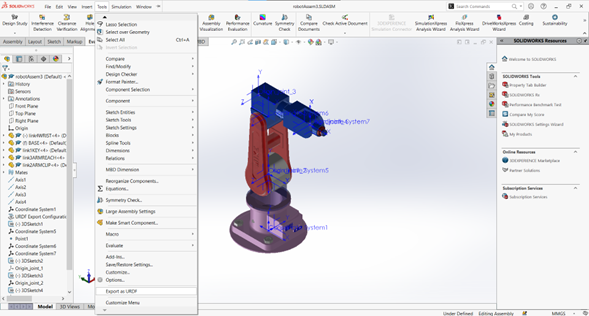
\includegraphics[width=0.7\textwidth]{img/urdfsolid.png}
	\caption{Modelo en SolidWorks}
	\label{fig:robotSolid}
\end{figure}
Una vez exportado el robot, se instaló el \textit{Windows Subsystem for Linux} (WSL) utilizando Visual Studio Code, fue aquí donde se llevó a cabo toda la simulación. A partir de esto, se creó un workspace llamado moveitws específicamente para organizar el proyecto. El paquete fue renombrado a robotassem3 para evitar errores relacionados con nombres que contienen mayúsculas.
\begin{figure}[H]
	\centering
	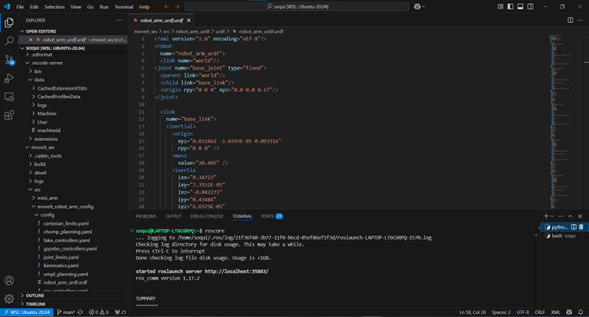
\includegraphics[width=0.7\textwidth]{img/wsl.png}
	\caption{Codigo}
	\label{wsl}
\end{figure}
Dentro del URDF se realizaron varios ajustes importantes: se corrigieron las rutas de las mallas e incluso se cambiaron los .stl a .dae, se definieron correctamente los joints entre cada link, y se agregaron los elementos necesarios para integrar con Gazebo, incluyendo el plugin de gazeboroscontrol y parámetros de colisión. Además, se definió un archivo YAML para los controladores (jointtrajectorycontroller.yaml), en el cual se configuraron los motores de las articulaciones (joint1 a joint4) usando controladores de tipo JointTrajectoryController.
\begin{figure}[H]
	\centering
	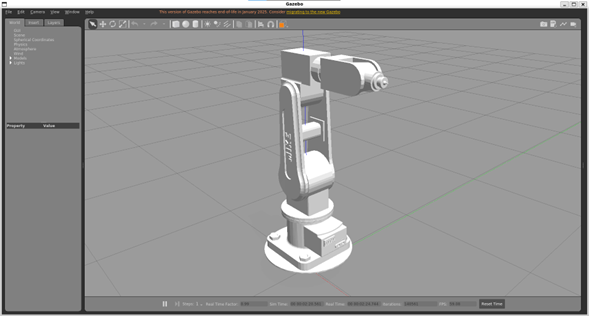
\includegraphics[width=0.7\textwidth]{img/gazebo.png}
	\caption{Modelo de Gazebo}
	\label{gazebo}
\end{figure}
Se diseñó un archivo launch (armurdf.launch) que permite lanzar el robot en un mundo vacío de Gazebo, cargar su descripción URDF, iniciar los controladores y visualizar su movimiento. En esta etapa, fue necesario ajustar los valores de posición (origin) y orientación (rpy) de los joints, ya que inicialmente el robot aparecía desarmado o con las piezas mal alineadas en Gazebo. Una vez corregido esto, el modelo se visualizó correctamente y pudo ser controlado mediante los controladores ROS definidos.
Posteriormente, se utilizó MoveIt Setup Assistant para importar el URDF y generar la configuración necesaria para planificación de movimientos. Se definieron los grupos de planificación, el end-effector (que no incluimos porque nuestro robot no tiene pinza, sólo una herramienta), los límites articulares y las poses del robot. A pesar de que el modelo no se visualizó correctamente en RViz, el sistema sí fue funcional: los joints respondieron al planificador y se pudieron probar trayectorias usando MoveIt.
\begin{figure}[H]
	\centering
	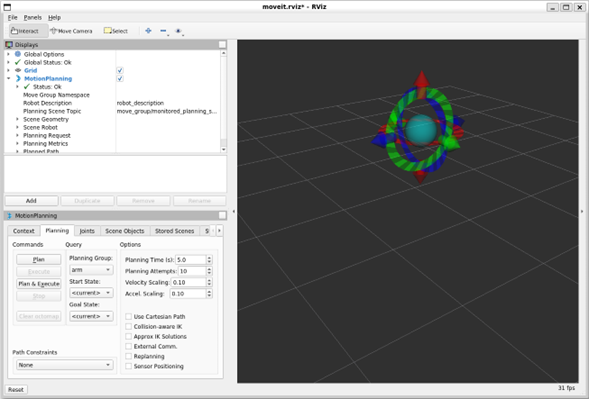
\includegraphics[width=0.7\textwidth]{img/rviz.png}
	\caption{RViz}
	\label{rviz}
\end{figure}
Durante todo el proceso, se enfrentaron dificultades técnicas como la incorrecta visualización inicial en Gazebo, problemas con los nombres de paquetes exportados desde SolidWorks, errores en la definición de joints y el problema que no pudo resolverse: la visualización en RViz. Sin embargo, tras realizar los ajustes necesarios, el robot fue simulado correctamente y se logró integrar con éxito a MoveIt para el control y planificación de sus movimientos.